Fitting the anomalous couplings one at a time while fixing the other couplings
to the Standard Model values, we get the following results:

%% [#1] INFO:Minization --  Including the following contraint terms in minimization: (n_ww_con,n_top_con,n_wjets_con,n_wz_con,n_zz_con,n_dy_con)
%% [#1] INFO:Fitting -- RooAddition::defaultErrorLevel(nll_cpdf_data_with_constr) Summation contains a RooNLLVar, using its error level
%% Minuit2Minimizer: Minimize with max iterations 3500 edmval 1 strategy 1
%% Minuit2Minimizer : Valid minimum - status = 0
%% FVAL  = -1570.82411436535926
%% Edm   = 4.46449224864883129e-07
%% Nfcn  = 107
%% n_dy  = 14.6556 +/-  12.1723(limited)
%% n_top  = 95.4423 +/-  40.2391(limited)
%% n_wjets  = 92.2872 +/-  37.241(limited)
%% n_ww  = 882.544 +/-  69.3925(limited)
%% n_wz  = 18.6031 +/-  3.71082(limited)
%% n_zz  = 10.5638 +/-  1.95431(limited)
%% x_par  = -1.70166e-05 +/-  0.0459015(limited)
%% Info in <Minuit2>: MnMinos Parameter is at Lower limit. : par = 0
%% Minos:  Parameter  is at Lower limit.
%% Minos: Lower error for parameter 0  :  -11.7306
%% Minos: Upper error for parameter 0  :  13.1518
%% Minos: Lower error for parameter 1  :  -40.5837
%% Minos: Upper error for parameter 1  :  40.7585
%% Minos: Lower error for parameter 2  :  -37.7355
%% Minos: Upper error for parameter 2  :  37.8638
%% Minos: Lower error for parameter 3  :  -69.0921
%% Minos: Upper error for parameter 3  :  69.7463
%% Minos: Lower error for parameter 4  :  -3.72203
%% Minos: Upper error for parameter 4  :  3.72179
%% Minos: Lower error for parameter 5  :  -1.95932
%% Minos: Upper error for parameter 5  :  1.95925
%% Minos: Lower error for parameter 6  :  -0.0418341
%% Minos: Upper error for parameter 6  :  0.0400667
%% [#1] INFO:Minization --  Including the following contraint terms in minimization: (n_ww_con,n_top_con,n_wjets_con,n_wz_con,n_zz_con,n_dy_con)
%% [#1] INFO:Fitting -- RooAddition::defaultErrorLevel(nll_cpdf_data_with_constr) Summation contains a RooNLLVar, using its error level
%% Minuit2Minimizer: Minimize with max iterations 3500 edmval 1 strategy 1
%% Minuit2Minimizer : Valid minimum - status = 0
%% FVAL  = -1570.83135328199637
%% Edm   = 4.15084504294644057e-06
%% Nfcn  = 88
%% n_dy  = 14.6504 +/-  12.1733(limited)
%% n_top  = 95.4387 +/-  40.2264(limited)
%% n_wjets  = 92.2811 +/-  37.2388(limited)
%% n_ww  = 882.543 +/-  69.3832(limited)
%% n_wz  = 18.6029 +/-  3.71081(limited)
%% n_zz  = 10.5638 +/-  1.95431(limited)
%% y_par  = -0.00441149 +/-  0.0726164(limited)
%% Info in <Minuit2>: MnMinos Parameter is at Lower limit. : par = 0
%% Minos:  Parameter  is at Lower limit.
%% Minos: Lower error for parameter 0  :  -11.7254
%% Minos: Upper error for parameter 0  :  13.1637
%% Minos: Lower error for parameter 1  :  -40.5865
%% Minos: Upper error for parameter 1  :  40.74
%% Minos: Lower error for parameter 2  :  -37.7432
%% Minos: Upper error for parameter 2  :  37.8552
%% Minos: Lower error for parameter 3  :  -69.142
%% Minos: Upper error for parameter 3  :  69.6855
%% Minos: Lower error for parameter 4  :  -3.72195
%% Minos: Upper error for parameter 4  :  3.72188
%% Minos: Lower error for parameter 5  :  -1.95926
%% Minos: Upper error for parameter 5  :  1.95931
%% Minos: Lower error for parameter 6  :  -0.068117
%% Minos: Upper error for parameter 6  :  0.0650093

%% [#1] INFO:Minization --  Including the following contraint terms in minimization: (n_ww_con,n_top_con,n_wjets_con,n_wz_con,n_zz_con,n_dy_con)
%% [#1] INFO:Fitting -- RooAddition::defaultErrorLevel(nll_cpdf_data_with_constr) Summation contains a RooNLLVar, using its error level
%% Minuit2Minimizer: Minimize with max iterations 3500 edmval 1 strategy 1
%% Minuit2Minimizer : Valid minimum - status = 0
%% FVAL  = -1578.23834759283022
%% Edm   = 8.49758369833005371e-06
%% Nfcn  = 88
%% n_dy  = 13.3317 +/-  12.1083(limited)
%% n_top  = 104.607 +/-  39.6112(limited)
%% n_wjets  = 85.6998 +/-  37.4251(limited)
%% n_ww  = 882.045 +/-  69.1339(limited)
%% n_wz  = 18.5701 +/-  3.71085(limited)
%% n_zz  = 10.5779 +/-  1.95427(limited)
%% y_par  = 0.0055573 +/-  0.17761(limited)
%% Info in <Minuit2>: MnMinos Parameter is at Lower limit. : par = 0
%% Minos:  Parameter  is at Lower limit.
%% Minos: Lower error for parameter 0  :  -10.4067
%% Minos: Upper error for parameter 0  :  13.1619
%% Minos: Lower error for parameter 1  :  -39.8342
%% Minos: Upper error for parameter 1  :  40.131
%% Minos: Lower error for parameter 2  :  -38.0097
%% Minos: Upper error for parameter 2  :  38.064
%% Minos: Lower error for parameter 3  :  -68.8477
%% Minos: Upper error for parameter 3  :  69.4766
%% Minos: Lower error for parameter 4  :  -3.72208
%% Minos: Upper error for parameter 4  :  3.72186
%% Minos: Lower error for parameter 5  :  -1.95931
%% Minos: Upper error for parameter 5  :  1.95918
%% Minos: Lower error for parameter 6  :  -0.181625
%% Minos: Upper error for parameter 6  :  0.137579

Systematic uncertainties were included in the fit as Gaussian
constraints.

Final exclusion limits for anomalous couplings are:
\begin{align}
  \lambda_{Z}: [-0.042,0.040]~95\%~\mathrm{C.L.}\\
  \Delta g^{Z}_1: [-0.068,0.065]~95\%~\mathrm{C.L.}\\
  \Delta\kappa_\gamma: [-0.18,0.14]~95\%~\mathrm{C.L.}\\
\end{align}

Figure~\ref{fig:contour} shows 2D confidence limit contour plots for
anomalous couplings.

\begin{figure}[tp]
  \centering
    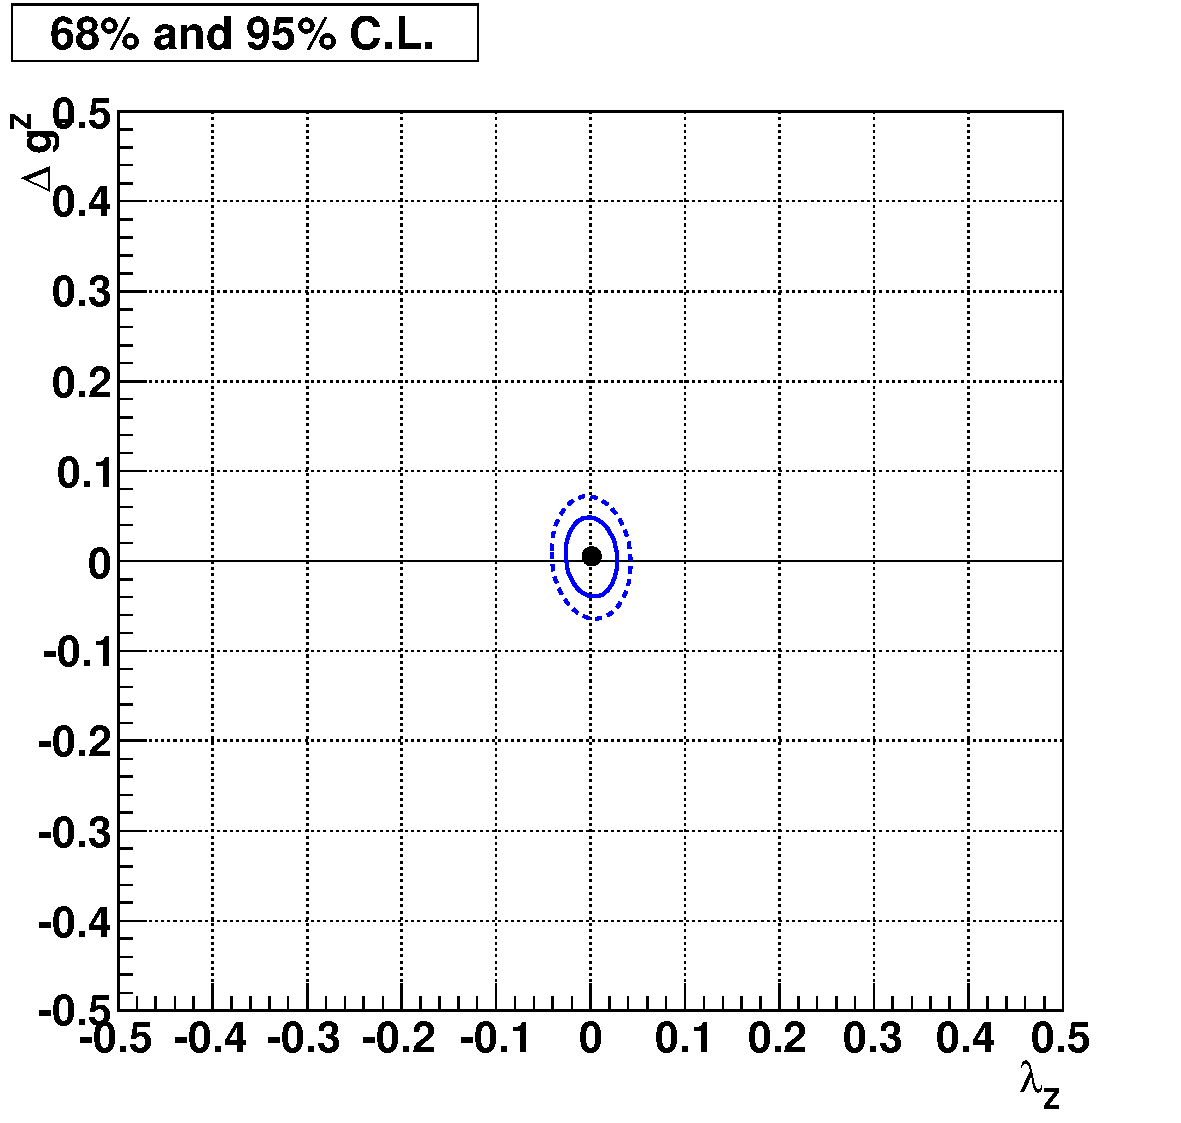
\includegraphics[width=0.7\textwidth]{figures/lz_dgz_contourplot}
    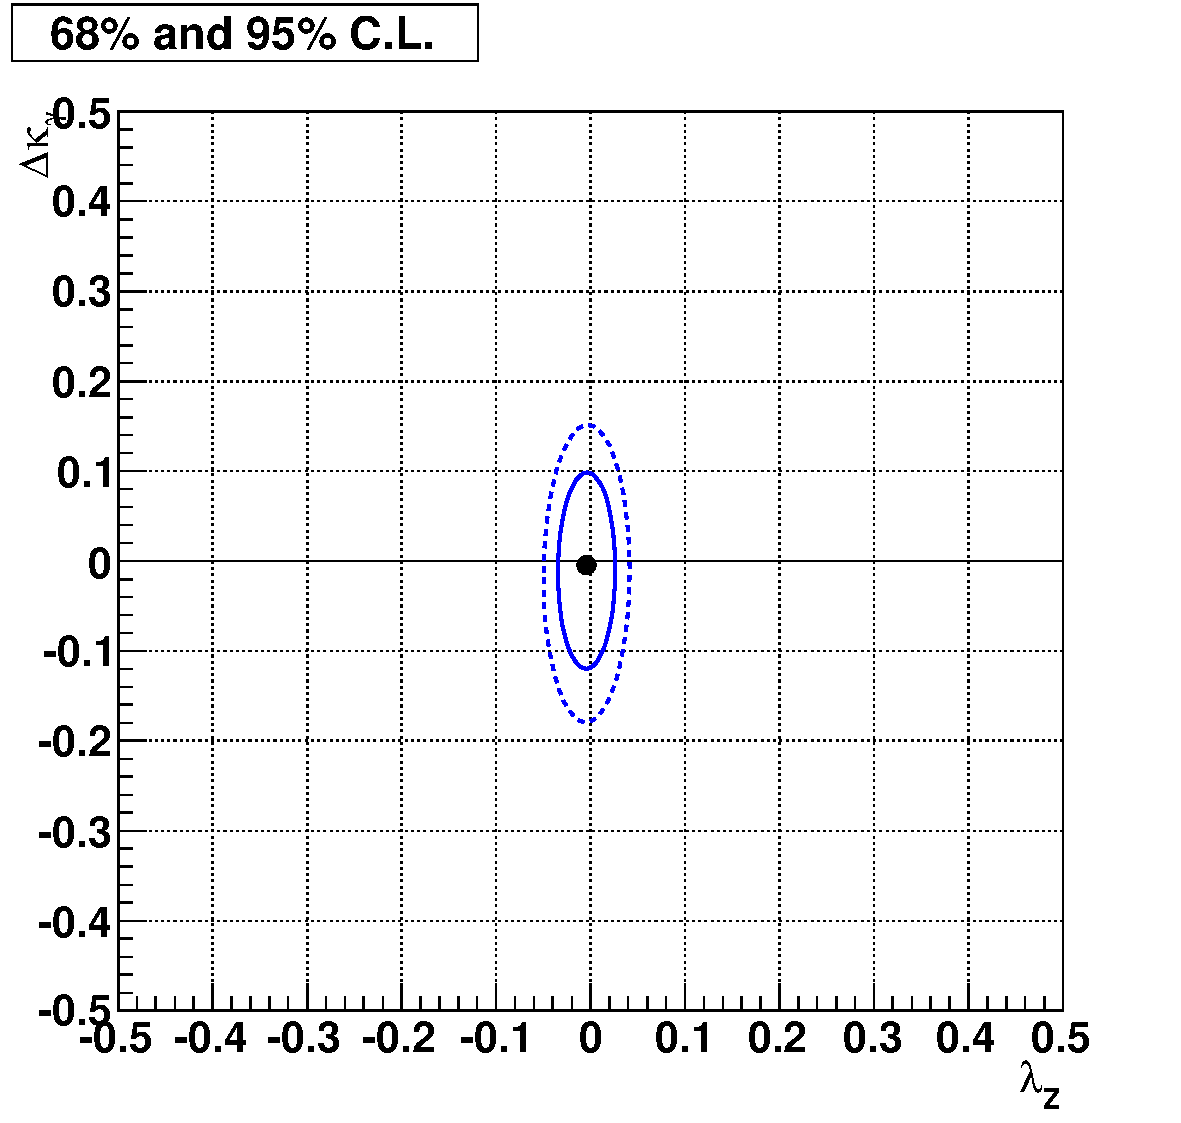
\includegraphics[width=0.7\textwidth]{figures/lz_dkg_contourplot}
  

  \caption[Contour plots for data] {aTGC 68\% and 95\% C.L. contour
    plots for a model without form factors for \intlumi of data.}
  \label{fig:contour}
\end{figure}

